\subsection{Component Investigation and Selection}
\subsubsection*{Airframe}
Given the aircraft presented previously, the most suitable design for this project is the FireFLY6. However, even under expensive modifications, it may not be able to meet requirements \textbf{R3} and \textbf{R4}. An alternative was to purchase a hobby airframe and design an aircraft to emulate the design of the FireFLY6.\\

The Skywalker X8 \cite{ref:x8} is a commonly used airframe that can easily be used to replicate the FireFLY6's motor configuration, and has been shown to be capable of up to 155km of flight \cite{ref:range}, which far exceeds the requirements for the UAV Challenge. In addition, the X8 is purpose designed to mount various sensors (such as a camera) to its frame, with large under canopy storage for components, and the best wingspan to weight ratio of the airframes researched for development.\\

Appendix \ref{sec:selection} presents a detailed analysis of several design options, comparing the purchase of various FireFLY6 models to several designs based on the X8. Estimations of the X8's flight performance was modeled using eCalc \cite{ref:ecalc}, a commonly used web tool in the aircraft building community for calculating the performance of aerial vehicles. This site has a vast collection of empirical data for motors, propellers, batteries and aircraft configurations and boasts an accuracy of $\pm$10\% for all calculations. The X8 configuration was shown to be the most suitable option, outperforming the FireFLY6 in cost, flight time, and manoeuvrability, with an expected payload of 3.5kg. Even if requirements are not met, this prototype will none the less form a strong basis for competing in the UAV Challenge and continued development \\


\subsubsection*{Flight Control}
The addition of a flight controller to the aircraft permits autonomous flight capabilities, including way point planning and motor control. The most viable (and well supported) options are the PixHawk \cite{ref:pixhawk}, APM 2.6 \cite{ref:ardupilot}, and PX4 \cite{ref:px4}. In order to achieve reliable and safe autonomous flight the controller must be fast and have sufficient storage for additional firmware/software to extend its capabilities. A comparison of each option may be found in \cite{ref:controller_comparison}, showing that given its larger memory storage, faster processor, and additional capabilities such as in-built gyroscopes and accelerometers, the PixHawk is the best choice for this project.

\subsubsection*{Controller Development}
The PixHawk flight controller has several flight control systems readily available for many types of aircraft (including fixed-wing and VTOL), but as of yet has no control system designed for a hybrid aircraft. Fortunately, the PX4 firmware (on which the PixHawk is based) is Open Source \cite{ref:ardupilotgit}, with several resources available \cite{ref:firmware1,ref:firmware2} to allow hobbyists and developers to customize the behaviour of their aircraft. The development of a hybrid flight controller is discussed further in Section \ref{sec:controller}.

\subsubsection*{Motor Configuration}
In order to achieve the novel transition system, the UAV's motors needed to be configured such that they could alternate between generating lift in VTOL flight, and propulsion in fixed-wing. Given the performance of the FireFLY6 a `Y' configuration was chosen, but rather than the FireFLY6's Y-6 (six motors positioned in the shape of a `Y'), a tri-coptor Y-3 configuration  was selected, as it would result in a lighter and cheaper aircraft. However, the aircraft was designed to be capable of being ``upgraded'' to a Y-6 configuration if the need arose.\\

The front motors were designed to be mounted such that they could be rotated forwards $90^{\circ}$ to facilitate the transition system and conversion to fixed-wing flight; the transition system is discussed further in Section \ref{sec:transition}. The rear motor mount system was designed to be tilted through the use of a servo-motor to enable the back motor to rotate, offsetting the uneven angular momentum generated by using only three motors.
		
\subsubsection*{Supports and Mounting}
The airframe was designed to incorporate a combination of off-the-shelf carbon fiber parts and 3D printed plastic parts to provide the frame needed to mount the motors, internal supports, and sensors. Carbon fiber poles were chosen to form the main support for the UAV's motors because of their excellent strength-to-weight ratio, and were fitted with specially designed 3D printed mounts to mate with the motors. The poles and internal systems were secured within the UAV using 3D printed housings.
	
\subsubsection*{Motors}
The motors selected needed to provide both efficient hover and minimal power draw while cruising in fixed wing mode. As such, the \textit{Turnigy SK3 3542 800kv} motors were chosen, as they are efficient, well priced, and well reviewed. In addition, they were also used by \cite{ref:fireflyinstruction} to fly approximately 155km.
	
\subsubsection*{Propellers}
Modelling using eCalc suggested that smaller propellers provide better performance in fixed wing flight (less weight and drag), but larger propellers are better suited for VTOL (more thrust), with modelling presented in Appendix \ref{sec:ecalc}. As such, two sets of propellers were purchased (11$\times$5.5 and 12$\times$6) in both plastic and carbon fiber, to perform testing on.
	
\subsubsection*{Servo-motors}
Servo-motors were required to make up the front transition system and the back yaw system. Both servos chosen were \textit{Turnigy TGY-4409MDs}, capable of 8.65kg.cm of torque at 5V, more than the required amount to overcome the force of the motors. 
		
\subsubsection*{Batteries}
The primary method for maximizing flight time and range is by reducing weight. \textit{Multistar 8000 mAh} batteries were selected as they have a much higher capacity-to-weight ratio than conventional Lithium Polymer batteries. The prototype UAV made use of two of these batteries connected in parallel, adding extra weight, but providing significantly greater power capacity.

\subsection{Overall Design}
Based on these discussions and design decisions, the initial prototype design for this project will use a PixHawk flight controller in a Skywalker X8 airframe, mounted with three motors in a tri-coptor configuration. The aircraft will also be fitted with a transition system, to rotate the front motors and enable the aircraft to fly in both VTOL and fixed-wing modes. Finally, the aircraft will be mounted with various sensors, discussed in Section \ref{sec:sensing}, including a camera and LiDAR, to provide sensing capabilities for planning, obstacle detection and autonomous flight.\\

Figure \ref{fig:hardwarearch} shows a high level overview of the hardware architecture planned for the current and future teams. Boxes coloured in gray are aspects of the design that were out of the scope of the \ID team and thus not fully implemented on the prototype UAV. The remaining components will be discussed in detail in the following sections.

\begin{figure}[!h]
	\centering
	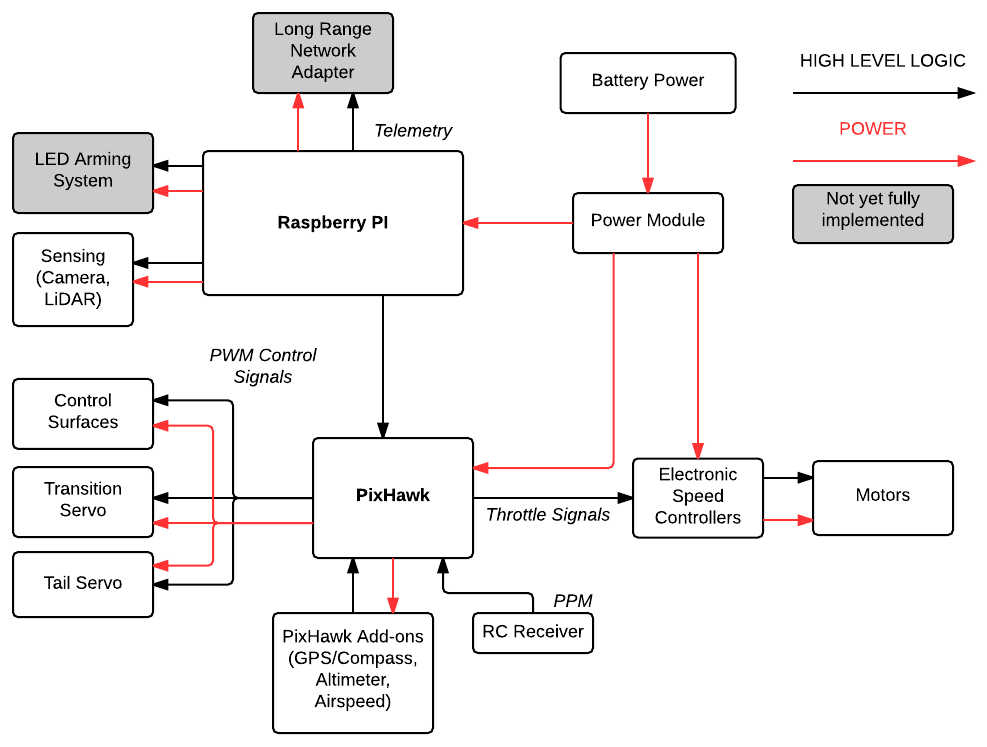
\includegraphics[width=380pt]{\IMAGEPATH /Diagrams/hardware}
	\caption{High level hardware architecture}
	\label{fig:hardwarearch}
\end{figure}

\subsection{Component and Design Validation}
Estimations of the flight performance for the overall design was modelled using eCalc \cite{ref:ecalc}, examples of the modelling process can be found in Appendix \ref{sec:ecalc}, with detailed performance estimations on the selected overall design shown in Figures \ref{fig:fixed} and \ref{fig:vtol}.\\

The configuration selected has an estimated 17.5 minutes of hover time, a surplus of time for the two vertical take off and landing manoeuvres required, thus leaving enough power to fulfill the 60km fixed wing flight requirement. Estimations for flight time and range during low power cruising fixed wing flight are not available through eCalc and must be done empirically. However, given the observed performance and capabilities of other aircraft based on the X8, the design of the prototype is expected to be suitable for the Challenge.\\

Additional calculations (see Appendix \ref{sec:stall}), verified fixed wing flight with the overall design. A worst case stall speed with the selected airframe's minimum coefficient of lift for level flight was determined to be at 45.5km/h. As the air will be forced over the wing by the motors during fixed wing flight, it is believed this should aid in creating additional lift.

\subsection{3D Printing}
In order to provide stable and robust mounting of all motors and mounting systems, 3D printing was utilized to create custom parts to fit within the X8 frame. The final versions of the major 3D printed parts (motor mounts, and the front and back mounting systems), parts that underwent the most designing, are presented below. Minor systems, and all design iterations for 3D printed parts, are provided in Appendix \ref{sec:print}.

\subsubsection*{Motor Mounts}
The motor mounts were required to secure each motor to its corresponding mounting pole. While the basic design was straight forward, several design iterations were required in order to develop a truly robust design. The carbon fiber pole is inserted into the motor mount, with cylindrical inserts (also 3D printed) providing additional strength, preventing the carbon fiber from being crushed in the event of over tightening the fasteners. Hose clamps were also used to ensure that an equally distributed squeezing force was applied from the mount to the pole.

\begin{figure}[!ht]
	\centering
	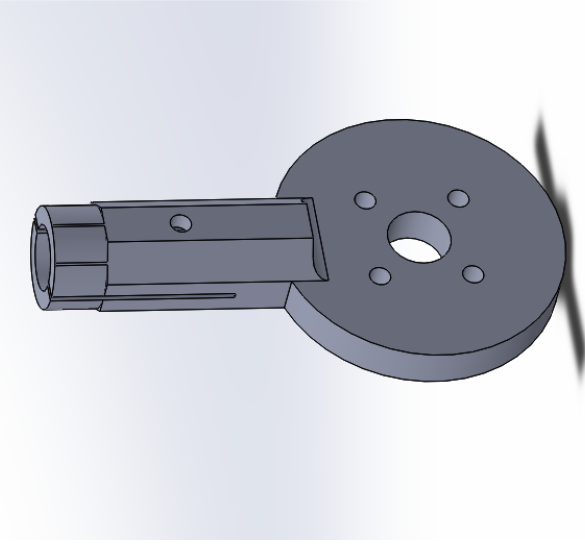
\includegraphics[width=160pt]{\IMAGEPATH Modelling/MotorMount3}
	\caption{Current iteration of the motor mount}
	\label{fig:designmotormount}
\end{figure}
	
\subsubsection*{Front Mounting System}
The front mounting system was required to incorporate the transition system, while also being stable enough to withstand disturbances associated with supporting two motors. As such, it was designed to fit completely within the Skywalker X8's front recess to ensure that the entire system was supported, and that any lateral load on the front mounting pole (i.e. incoming wind) would be transferred through the entire aircraft and not just the front mounting system itself. A servo is also mounted here to facilitate the transition system.

\begin{figure}[!ht]
	\centering
	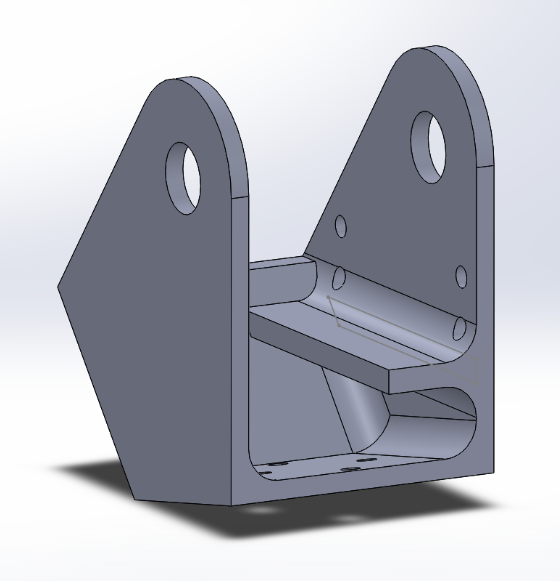
\includegraphics[width=150pt]{\IMAGEPATH Modelling/FrontMount3}
	\caption{Current iteration of the front mounting system}
	\label{fig:designfrontmount}
\end{figure}
	
\subsubsection*{Back Mounting System}
The back mounting system was required to incorporate the yaw servo-motor system and also keep the back motor pole perpendicular to the front motor pole. A multi-webbed design was developed to keep the pole aligned, in addition to the supplied Skywalker X8 tail ring support. Housing for the yaw servo-motor was built into the system to ensure backlash-free mating between the gear and the pole.\\

\begin{figure}[!ht]
	\centering
	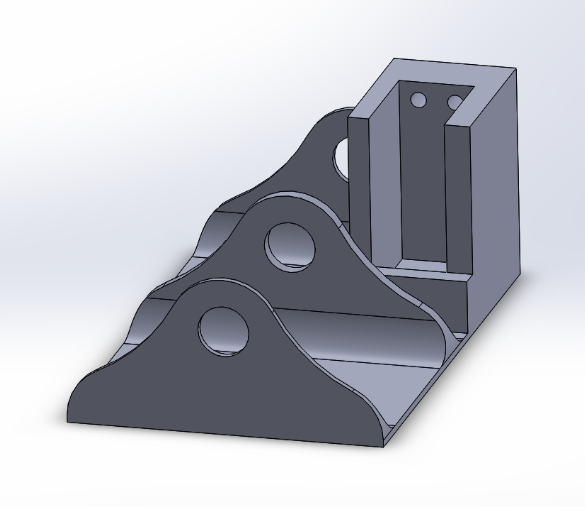
\includegraphics[width=150pt]{\IMAGEPATH Modelling/BackMount2}
	\caption{Current iteration of the back mounting system}
	\label{fig:designbackmount}
\end{figure}

\subsection{Calibration}
\subsubsection*{Motor and Propeller Balancing}
To eliminate potential vibrations generated from propellers, each propeller was first balanced by either adding mass (using tape, or similar) or removing mass (shaving off material) from either side. A non-destructive method was preferred, so small pieces of tape were added to the propellers using the balancing apparatus shown in Figure \ref{fig:propbalancing} to ensure the mass distribution was equal. The propellers were tested using the Seismograph Android app before and after balancing, which showed a large decrease in vibrations.
\begin{figure}[!ht]
	\centering
	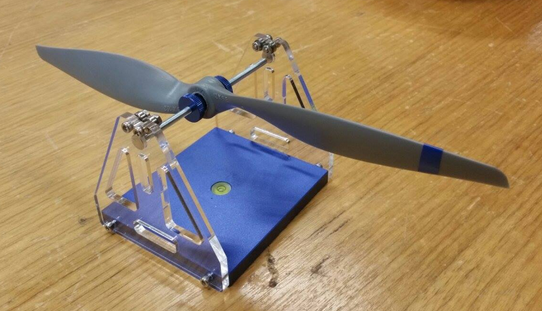
\includegraphics[width=300pt]{\IMAGEPATH /Prototype/prop_balancer}
	\caption{Propeller balancing apparatus, with tape added to propeller to improve balance}
	\label{fig:propbalancing}
\end{figure}

\subsubsection*{Mass Balancing}
The center of gravity (CoG) of the UAV may be changed by repositioning the batteries (the heaviest items to be carried). The position of the CoG needed to meet the following specifications:

\begin{itemize}
	\item The center of mass had to be at the center of thrust of the VTOL. Due to the triangular nature of the propeller setup, this meant the CoG would be one third of the distance from the front propellers to the back propeller (approximately 30cm from the front motors), resulting in an equal moment about the center of gravity. This would allow all motors to produce the same amount of thrust without causing an undesired tilt in the UAV.
	\item The center of mass also had to be at the center of lift, which for the Skywalker X8 is given as 44cm from the nose of the aircraft \cite{ref:x8kit}. The distance of the front motors from the nose of the aircraft is approximately 14cm. With the center of mass positioned 30cm from the front motors, the center mass and center of lift are coincident.
\end{itemize}
	
\subsubsection*{Electronic Speed Controller Calibration}
Following the manufacturer's manual, the receiver and PixHawk signals were calibrated into the electronic speed controllers (ESCs) by setting a minimum and maximum motor throttle. This allowed for the maximum throttle range of the controller to be used, and most importantly, the use of the motors at full speed.

\subsubsection*{PixHawk Calibration}
Many parameters on the PixHawk required setting and calibration, such as fail safes, input directions, output maximums and minimums, and radio end points. The inbuilt compass and accelerometer required tuning each time the internal configuration of the aircraft changed in order to ensure level flight. This is achieved through performing specific calibration points in the open source program, Mission Planner. A once off power module voltage and radio calibration were also required to ensure correct battery monitoring. 


\subsubsection*{PID Tuning}
The PixHawk comes with in-built PID parameters that may be tuned for specific applications. Basic tuning was performed for the UAV by first setting the roll, pitch, and throttle gains and sensitivities to ensure stable and responsive flight controls. The UAV was then launched (without wings) and placed into an auto-tune flight mode, allowing the PixHawk to perform a series of pre-programmed maneuvers to find the best possible PID values for the custom aircraft.\\

\begin{figure}[!ht]
	\centering
	\begin{subfigure}{.5\textwidth}
		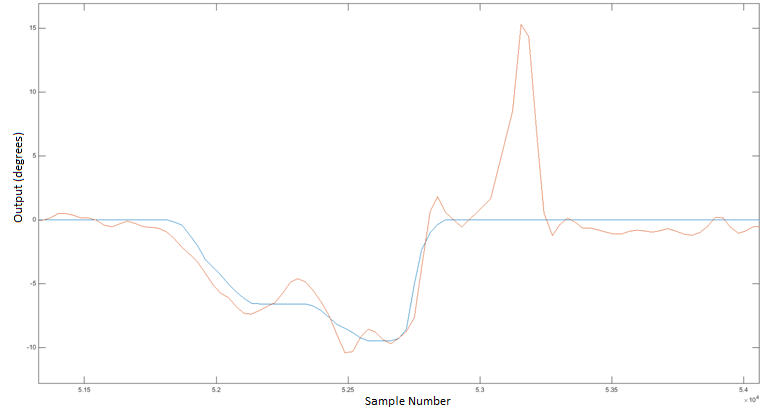
\includegraphics[width=250pt]{\IMAGEPATH /Data/untuned}
		\caption{Untuned roll with significant overshoot}
		\label{fig:untunedroll}
	\end{subfigure}%
	\begin{subfigure}{.5\textwidth}
		\centering
		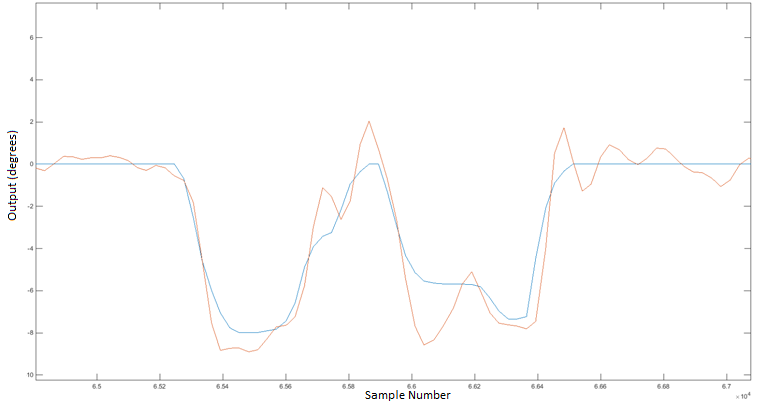
\includegraphics[width=250pt]{\IMAGEPATH /Data/tuned}
		\caption{Tuned roll}
		\label{fig:tunedroll}
	\end{subfigure}
	\caption{Comparison of tuned and untuned flight performance; Blue = desired response, Red = measured response}
	\label{fig:tune1}
\end{figure}

Figure \ref{fig:tune1} shows log data collected by the PixHawk during the tuning flight. Figure \ref{fig:untunedroll} shows the performance of the UAV before tuning, and Figure \ref{fig:tunedroll} shows its performance after tuning, showing that while the response is still quite noisy, tuning has reduced the intensity of overshooting. Figure \ref{fig:tune2} shows the results of a second flight, this time with the UAV being fitted with wings halfway through the flight. With the wings attached the inertia, disturbances and weight of the UAV changed significantly; without wings, the UAV's roll (red) shows light noise and small overshoots, while after the wings were added noise increases significantly. However, the altitude response (yellow) of the aircraft remains stable, indicating that the aircraft still performs well when fitted with wings.

\begin{figure}[!ht]
	\centering
	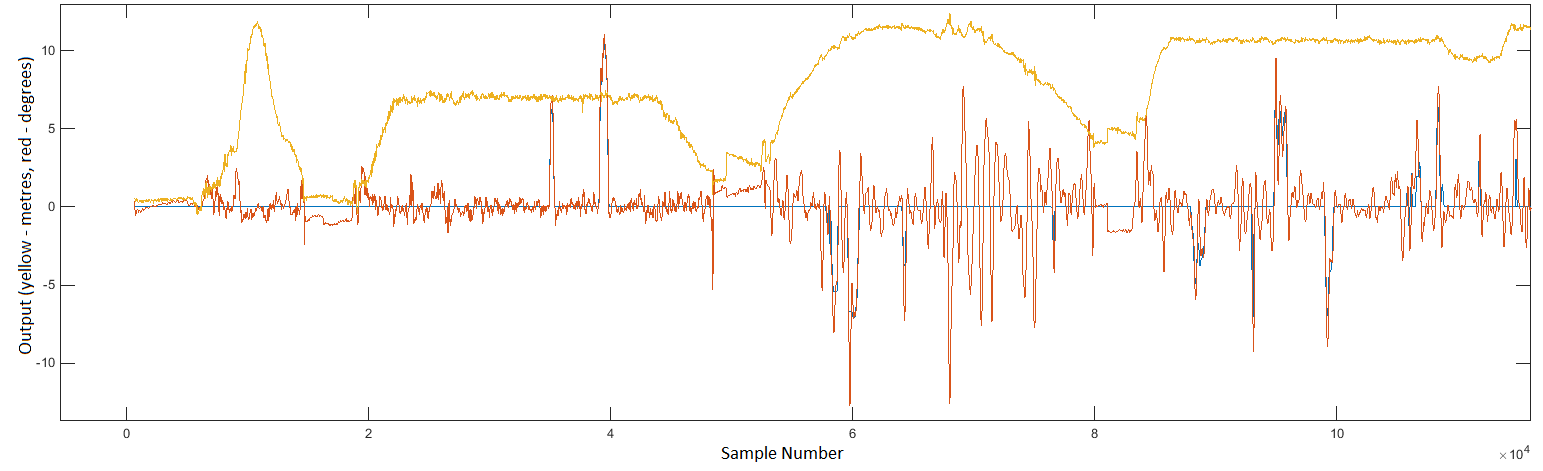
\includegraphics[width=500pt]{\IMAGEPATH /Data/tune_wings}
	\caption{Left half: Without wings. Right half: With wings.\\ Orange = Altitude (meters), Red = Roll (degrees)}
	\label{fig:tune2}
\end{figure}